\chapter{Solutions}
Il y a  plusieurs pistes de solutions afin de résoudre ce problème. Un end node visible par un noeud isolé peut etre redefinie comme une passerelle $\rightarrow$ On définit donc une \textit{LoRa} Gateway (noté LGW à travers le document)
Il y a donc une redéfinition des acteurs :
\begin{itemize}
\item LoRaWAN Gateway (LWGW)
\item LoRa Gateway 
\item Isolated Node (IN)
\end{itemize}

On aurais la possibilité d'avoir deux modes : 
\begin{itemize}
\item Mode proxy : La LoRaGateway fait un relai en aveugle des données des noeuds Isolés .
\item Mode concentrateur : La LoRaGateway collecte les données des Noeuds Isolés.
\end{itemize}
Il ya tout de même quelque problèmes pour le mode Proxy. 
En effet il y a une certaine compléxité de la mise en oeuvre. Que ce soit au niveau de l'écoute et la captures des échanges par des end-nodes mais aussi de la capture par le End Node de message du Noeud isolé, ou encore de la capture par le End Node de message à destination du Noeud isolé. Il y a aussi une certaine compléxité au niveau de la gestion des synchronisation en fonction des classes energetique des objets. En classez C, le problème se revele pendant les phases démission du End-Node. En classe A et B lors dez la gestion multiple des slots de réception par le un End Node. Il y a un derniere aspect qui est pratique, en effet les bibliothèques, on écoute et collecte des message sans en etre le destinataire. Il y aurais deux solutions pour pallier à cela, soit la mise en place d'un mode promiscuité, soit d'un recodage complet de la spécification.


Ici nous allons nous intéréssé surtout à l'ensemble des algorithmes qui décrive le fonctionnement du mode d'échanges classique entre une LGW et un IN, afin des les appliquer en simulation, puis de réaliser la mise en oeuvre/applications de ceux-ci.

\newpage
\section{Algorithme}


L'ensemble des messsages du système sont de la forme :

\begin{center}
\texttt{< message\_type , source , destination , data >}
\end{center}

On distingue donc plusieurs messages dans le système. On considère qu'à chaque message correspond une fonction portant le nom du message, initialisant le type et la source du message, et prenant en paramètre la destination et les données.

\subsection{les messages IN -> LGW}
\begin{itemize}
    \item les messages \texttt{discover}
    \begin{itemize}
      \item message mis en place pour la découverte d'une \texttt{LGW} par un \texttt{IN}
      \item \texttt{destination = udef} : en broadcast
      \item \texttt{data = udef} : aucune info
    \end{itemize}
    \item les messages \texttt{pair}
    \begin{itemize}
      \item message d'apairage d'un IN sur une LGW
      \item \texttt{data = udef} : aucune info
    \end{itemize}
    \item les messages \texttt{data\_response}
    \begin{itemize}
      \item réponse à une demande de données de la part d'une LGW
    \end{itemize}
\end{itemize}

\subsection{les messages LGW -> IN}
Pour l'ensemble des messages LoRa issus de la \texttt{LGW} la partie data est structurée ainsi :

\begin{itemize}
  \item \texttt{answer\_frequency} : fréquence sur laquelle l'\texttt{IN} doit répondre
  \item \texttt{next\_slot} : délai d'ici la prochaine fenêtre d'écoute
  \item \texttt{next\_duration} : temps fixé de la prochaine fenêtre d'écoute
  \item \texttt{next\_frequency} : fréquence de la prochaine fenêtre d'écoute
  \item \texttt{data} : espace de données spécifiques à l'échange
\end{itemize}

Le message devient donc :

\begin{center}
\texttt{< message\_type , source , destination , answer\_frequency , next\_slot , next\_duration , next\_frequency , data>}
\end{center}

Les différents messages \texttt{LGW} $\rightarrow$ \texttt{IN} sont donc :
\begin{itemize}
    \item les messages \texttt{candidate} %\textbf{(ce nom ne me plait pas !!!)}
    \begin{itemize}
      \item message de réponse d'une \texttt{LGW} après réception d'un \texttt{discover} d'un \texttt{IN}
      \item \texttt{data = udef} : aucune info
    \end{itemize}
    \item les messages \texttt{data\_request}
    \begin{itemize}
      \item message de demande de données
      \item \texttt{data = udef} si une seule donnée disponible ou \texttt{data = requested\_data} dans le cas de donnés multiples
    \end{itemize}
\end{itemize}

\section{Liste des fonctions utilisées}

\subsection{Fonction d'émission}

\texttt{void sendLora(frequency , message)}

\subsection{Fonction de réception}

la fonction \texttt{listen} écoute sur la fréquence \texttt{frequency} un temps définit par \texttt{time}. Le prototype de cette fonction est :

\begin{center}
\texttt{(message,time) listen(frequency , source , message\_type , time\_listen)}
\end{center}

les valeurs des paramètres de cette fonction sont :
\begin{itemize}
  \item \texttt{frequency} : fréquence d'écoute
  \item \texttt{source} : id de l'émetteur du message
  \begin{itemize}
    \item \texttt{source = udef} : écoute de tous les n{\oe}uds sur la fréquence définie
  \end{itemize}
  \item \texttt{message\_type} : type de message attendu
  \begin{itemize}
    \item \texttt{message\_type = udef} : écoute de tous les types de messages
  \end{itemize}
  \item \texttt{time\_listen} : durée de la fenêtre de réception
  \begin{itemize}
    \item \texttt{time\_listen = udef} : fenêtre infinie
  \end{itemize}
\end{itemize}

Valeurs de retour :

\begin{itemize}
  \item \texttt{message} message reçu
  \begin{itemize}
    \item passage du message dans sa totalité
    \item \texttt{message == udef} : pas de réception respectant les contraintes
  \end{itemize}
  \item \texttt{time} temps restant basé sur \texttt{time\_listen}
  \begin{itemize}
    \item \texttt{time == udef} : dans le cas de \texttt{time\_listen = udef}
  \end{itemize}
\end{itemize}

\section{Algorithme 1 - 1}

\subsection{Algorithme des \texttt{IN}}

\begin{algorithm}
\caption{Initialisation des variables de communication}\label{alg:intvar}
\begin{algorithmic}[1]
\Procedure{$init\_var$}{msg}
\State $lgw \leftarrow msg.source$
\State $freq\_send \rightarrow msg.answer\_frequency$
\State $next\_time \leftarrow msg.next\_slot$
\State $timer \leftarrow msg.next\_duration$
\State $freq\_listen \leftarrow msg.next\_frequency$
\EndProcedure
\State
\Procedure{$flush\_var$}{~}
\State $lgw \leftarrow udef$
\State $msg \leftarrow udef$
\State $next\_time \leftarrow udef$
\State $timer \leftarrow timer\_disco$
\State $freq\_listen \leftarrow freq\_disco$
\State $freq\_send \leftarrow freq\_disco$
\EndProcedure
\end{algorithmic}
\end{algorithm}


\begin{algorithm}
\caption{Algorithme IN 1-1}\label{alg:in1-1}
\begin{algorithmic}[1]
\While{$(true)$}
  \State $flush\_var()$
  \State \Comment{------------------------------------------------------- \textit{phase d'apairage}}
  \While{$(msg = udef)$}
    \State $sendLora(freq\_listen,discover(udef,udef))$
    \State $(msg,t) = listen(freq\_send,udef,candidate,timer + rnd())$
  \EndWhile
  \State $initVar(msg)$
  \State $sendLora(freq\_send,pair(lgw,udef))$
  \State
  \State \Comment{----------------------------------------------\textit{Phase d'échanges}}
  \While{$(lgw != udef)$}
    \State $sleep(next\_time)$
    \State $(msg,t) = listen(freq\_send,lgw,data\_request,timer)$
    \If{$msg != udef$}
      \State $initVar(msg)$
      \State $sendLora(freq\_send,date\_response(lgw,local\_data)$
    \Else
      $flush\_var()$
    \EndIf
  \EndWhile
\EndWhile
\end{algorithmic}
\end{algorithm}

\subsection{Algorithme des \texttt{LGW}}

\begin{algorithm}
\caption{Initialisation des variables de communication}\label{alg:initvarlg}
\begin{algorithmic}[1]
\Procedure{$init\_var$}{~}
\State $freq\_send \rightarrow chose()$
\State $timer \leftarrow chose()$
\State $freq\_listen \leftarrow chose()$
\State $freq\_next \leftarrow chose()$
\EndProcedure
\State
\Procedure{$flush\_var$}{~}
\State $timer \leftarrow timer\_disco$
\State $freq\_listen \leftarrow freq\_disco$
\State $freq\_send \leftarrow freq\_disco$
\State $in \leftarrow udef$
\EndProcedure
\end{algorithmic}
\end{algorithm}

\begin{algorithm}
\caption{Algorithme lgw 1-1}\label{alg:lgw1-1}
\begin{algorithmic}[1]
\State $LoRaWAN\_join()$
\State $flush\_var()$
\While{$(true)$}
  \If{$(in == udef)$}
    \State $(msg,t) = listen(freq\_listen,udef,discover,timer)$
  \EndIf
  \If{$(msg != udef)$}
    \State $in \leftarrow msg.source$
    \State $init\_var()$
    \State $sendLora(freq\_send,candidate(in,freq\_listen,slot,duration,freq\_next,udef)$
    \State $(msg,t) = listen(freq\_listen,in,pair,timer)$
    \If{$(msg == udef)$}
      \State $flush\_var()$
    \EndIf
  \EndIf
  \If{$(in != udef)$}
    \State $init\_var()$
    \State $sendLora(freq\_send,data\_request(in,freq\_listen,slot,duration,freq\_next,udef)$
    \State $(msg,t) = listen(freq\_listen,in,data\_response,timer)$
    \If{$(msg != udef)$}
      \State $send\_lora\_data(id + ":" + local\_data + ";" + in + ":" + msg.data)$
    \Else
      \State $send\_lora\_data(id + ":" + local\_data + ";" + in + ":" + udef)$
      \State $flush\_var()$
    \EndIf
  \EndIf
\EndWhile
\end{algorithmic}
\end{algorithm}

\newpage
\subsection{Algorithme k/1 : k IN <-> 1 LGW}
Ici le seul changement qui opère est celui d'enregistrement de plusieurs noeuds isolés.
\begin{algorithm}
\caption{Algorithme lgw 1-1}\label{alg:lgwk-1}
\begin{algorithmic}[1]
\State $LoRaWAN\_join()$
\State $flush\_var()$
\While{$(true)$}
  \If{$(in == udef)$}
    \State $(msg,t) = listen(freq\_listen,udef,discover,timer)$
  \EndIf
  \If{$(msg != udef)$}
    \State $in \leftarrow msg.source$
    \State $init\_var()$
    \State $sendLora(freq\_send,candidate(in,freq\_listen,slot,duration,freq\_next,udef)$
    \State $(msg,t) = listen(freq\_listen,in,pair,timer)$
    \If{$(msg == udef)$}
      \State $flush\_var()$
    \EndIf
  \EndIf
  \If{$(in != udef )$}
 	 \If{$(in NOT in tabRegisteredIN )$}
 	 	\State $ tabRegisteredIN.append(in)$
 	 \EndIf
  	  \State $init\_var()$
  	  \State $sendLora(freq\_send,data\_request(in,freq\_listen,slot,duration,freq\_next,udef)$
  	 \State $(msg,t) = listen(freq\_listen,in,data\_response,timer)$
   	 \If{$(msg != udef)$}
    	  \State $send\_lora\_data(id + ":" + local\_data + ";" + in + ":" + msg.data)$
    	\Else
    	  \State $send\_lora\_data(id + ":" + local\_data + ";" + in + ":" + udef)$
    	  \State $flush\_var()$
    \EndIf
  \EndIf
\EndWhile
\end{algorithmic}
\end{algorithm}
\newpage
\section{Chronogrammes}
\subsection{Phase de découverte et d'enregistrement}
\begin{figure}[!ht]
\centering
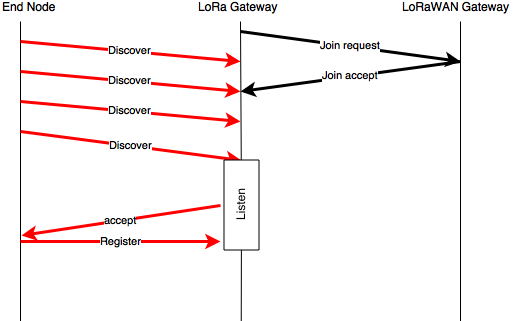
\includegraphics[scale=0.6]{Discovery.png} 
\caption{Phase de découverte}
\end{figure}
\subsubsection{Coté Isolated node}Au début le noeud isolé se reveille, il envoie des messages \textbf{Discover}. Si une \textit{LoRa} Gateway répond par un message \textbf{Accept} le noeud répond alors avec un message  \textbf{Register} pour confirmer son appairage avec la \textit{LoRa} Gateway.
\subsubsection{Coté LoRa Gateway}
La \textit{LoRa} Gateway avant toute opération avec n'importe quel élement de l'environnement doit s'appairer avec une gateway \textit{LoRaWAN} avec la requete  \textbf{Join Request}.
\subsubsection{Coté LoRaWAN Gateway}
La gateway \textit{LoRaWAN} executé un déroulement normal. Elle répond aux requetes join avec un message  \textbf{Join Accept}
\newpage
\subsection{Phase de collecte}
\begin{figure}[!ht]
\centering
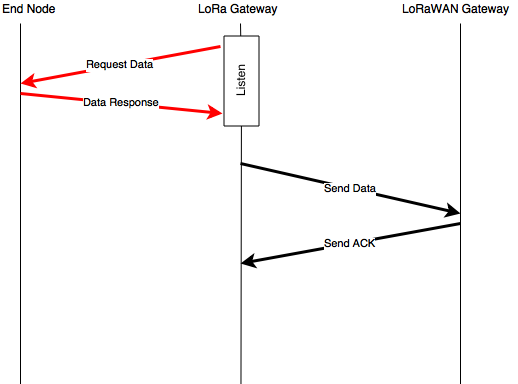
\includegraphics[scale=0.6]{Collect.png} 
\caption{Phase de collecte}
\end{figure}

\subsubsection{Coté Isolated node} Le noeud se reveille à un slot prévu entre la \textit{LoRa} Gateway et le noeud. Tout ceci afin de recevoir la demande de donnée de la part de la gateway \textit{LoRa}. Le noeud répond avec les données dans un message nommé  \textbf{Data Response}.
\subsubsection{Coté LoRa Gateway}
La \textit{LoRa} Gateway va se reveiller pour collecter les données des noeuds qui lui sont accroché. Elle envoit donc un message  \textbf{Request Data} . \\
Mode Concentrateur : Une fois que toutes les données sont reçues, la Gateway assemble les données et envoie à la  \textit{LoRaWAN} gateway. \\
Mode Proxy : Une fois que toutes les données sont reçues, la Gateway usurpe chaque isolated node et envoie les données à la  \textit{LoRaWAN} gateway. Pour finir par envoyé ces propres données.
\subsubsection{Coté LoRaWAN Gateway}
La \textit{LoRaWAN} Gateway accuse la reception des données envoyées par la gateway \textit{LoRa}.
\textbf{Send ACK}
